%% ============================================================================
%% SUPPORTING INFORMATION for
%% "Oblate Spheroid Excitation Theory (OSET): a unified, lattice-free
%%  foundation for plastic deformation from which dislocations emerge as
%%  collective excitations"
%% A. Linda, K.A. Padmanabhan -- prepared for Acta Materialia
%%
%% This document collects, in full numerical detail, every comparison and
%% validation result that is summarised in condensed form in the main text.
%% Sections (and their figures) are ordered to match the sequence in which
%% they are first cited from the main text, not by topic:
%%   S1  Eshelby tensor component S_1313 (cited early, Sec. numeval)
%%   S2  Stacking-fault energy predictions across crystal systems
%%   S3  Grain-boundary energy verification across crystal systems (FCC/BCC/HCP)
%%   S4  Supplementary derivation figures: hardening and occupation factor
%%   S5  Full validation against the original Padmanabhan et al. (1996) data
%%   S6  Independent post-1996 literature validation; Unified Rate Equation
%%       applied across material classes
%%   S7  Full 41-system comparison with Harisankar & Padmanabhan (2025)
%%
%% Build: pdflatex -> pdflatex
%% ============================================================================
\documentclass[11pt]{article}

\usepackage[margin=1in]{geometry}
\usepackage{amsmath,amssymb,amsfonts}
\usepackage{graphicx}
\usepackage{booktabs}
\usepackage{longtable}
\usepackage[hidelinks]{hyperref}
\usepackage{natbib}

\graphicspath{{figures/}}

\renewcommand{\thesection}{S\arabic{section}}
\renewcommand{\thetable}{S\arabic{table}}
\renewcommand{\thefigure}{S\arabic{figure}}

\newcommand{\OSTZ}{\textsc{ostz}}
\newcommand{\OSET}{\textsc{oset}}
\newcommand{\dF}{\Delta F_0}
\newcommand{\g}{\gamma_0}
\newcommand{\eps}{\varepsilon_0}
\newcommand{\half}{\tfrac{1}{2}}

\title{Supporting Information\\[4pt]
\large Oblate Spheroid Excitation Theory (\OSET): a unified, lattice-free
foundation for plastic deformation from which dislocations emerge as
collective excitations}
\author{Albert Linda \and K.A. Padmanabhan}
\date{}

\begin{document}
\maketitle

This document collects, in full numerical detail, every quantitative
comparison and validation result referenced in the main text. The main
text states the headline agreement for each claim and refers to the
corresponding table here for the complete underlying numbers; equation
numbers from the main text are given explicitly (e.g.\ ``Eq.~60 of the
main text'') and table numbers here are prefixed ``S''.

\tableofcontents

% =============================================================================
\section{Eshelby tensor component $S_{1313}$}
\label{si:s1313}

The shear constraint factor $\beta_1=1-2S_{1313}$ used throughout the
main text (Eshelby tensor numerical evaluation section) depends on
both the inclusion aspect ratio $\alpha=c/a$ and Poisson's ratio
$\nu$. Figure~\ref{si:fig:s1313}
plots this dependence explicitly across the full range of $\alpha$,
marking the thin-disk limit and the $\alpha=1/2$ value adopted for
the \OSTZ\ throughout this paper.

\begin{figure}[htbp]
\centering
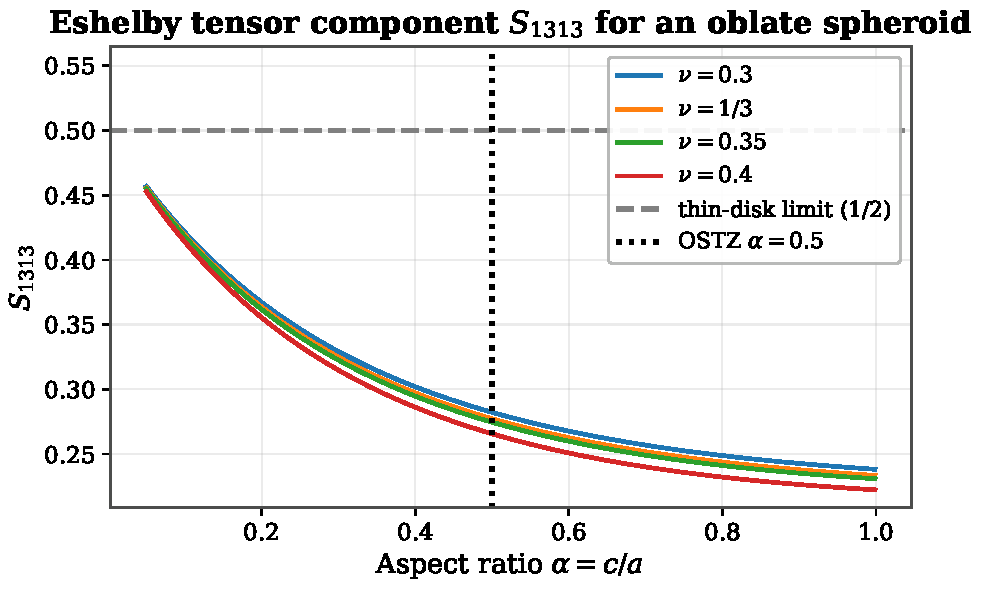
\includegraphics[width=0.8\linewidth]{fig_S1313.pdf}
\caption{Eshelby oblate-spheroid shear component $S_{1313}$ as a
function of aspect ratio $\alpha=c/a$, for several values of
Poisson's ratio $\nu$ spanning the range relevant to metals. The
thin-disk limit ($S_{1313}\to1/2$) and the aspect ratio
$\alpha=0.5$ used throughout this paper (giving $\beta_1=1-2S_{1313}$)
are marked.}
\label{si:fig:s1313}
\end{figure}

% =============================================================================
\section{Stacking-fault energy predictions across crystal systems}
\label{si:sfe}

Eq.~60 of the main text (stacking-fault energy) gives
$\gamma_\text{SF}=(\sqrt3-1)\beta_1\g^2GW/3$. The shear eigenstrain
$\g$ is the \emph{ideal (intrinsic) shear strain} of the material, that
is, the relaxed engineering shear strain $s_m$ at the maximum of the
first-principles shear stress--strain curve on the primary slip system.
We take $\g$ directly from the DFT compilation of
\citet{S_ogata2004} (their Table~II), an independent source, with
no fitting. An earlier version of this table instead fixed $\g=0.12$
(the Cu value) for every metal; that single universal constant is the
origin of the former large Al, Ni and Ag discrepancies. With the
literature $\g$ and $W=b$ (and $\beta_1^\text{eff}=1$) the stacking-fault
energy carries no adjustable parameter and reproduces experiment to
within a factor of about $2$ to $3$ (Table~\ref{si:tab:sfe}). We do not
tune $\g$ to improve the agreement. The residual scatter (Ag high, Al
low) reflects a known limitation of the isotropic-elastic scaling
$\gamma_\text{SF}\propto\g^2Gb$, which captures only part of the true
spread: the measured Al/Ag SFE ratio (about $10$) exceeds what $\g^2$
alone (about $1.9$) can supply, with the missing factor residing in the
anisotropic $\gamma$-surface shape beyond the single-eigenstrain OSTZ.

The numerical comparison itself, $\gamma_\text{SF}^\text{OSET}$ versus
the experimental/DFT value for every metal, is shown in the left
panel of Figure~\ref{si:fig:materials}, so we do not repeat it as a table.
Table~\ref{si:tab:sfe} instead lists only the \emph{literature input
values} that enter the prediction (the ideal shear strain $\g$) together
with the comparison target and its source, so that every number used is
traceable.

\begin{table}[htbp]
\centering
\caption{Literature inputs and comparison targets for the
crystal-interior predictions of Figure~\ref{si:fig:materials}. The OSTZ
eigenstrain $\g$ is the relaxed ideal shear strain $s_m$ on the primary
slip system, taken directly (no fitting) from
\citet{S_ogata2004}, Table~II. The stacking-fault energy
target is the measured/DFT value with its source; $G$, $b$, $\nu$ are
the same handbook values used throughout. BCC metals have no single
well-defined stacking fault, so no SFE target is assigned.}
\label{si:tab:sfe}
\begin{tabular}{llccc l}
\toprule
Metal & Struct. & Slip system & $\g$ (Ogata 2004) & $\gamma_\text{SF}$ target (mJ/m$^2$) & Source \\
\midrule
Cu & FCC & $\{111\}\langle112\rangle$ & 0.137 & 45  & \citep{S_gallagher1970}\\
Al & FCC & $\{111\}\langle112\rangle$ & 0.200 & 166 & \citep{S_gallagher1970}\\
Ni & FCC & $\{111\}\langle112\rangle$ & 0.140 & 125 & \citep{S_gallagher1970}\\
Ag & FCC & $\{111\}\langle112\rangle$ & 0.145 & 16  & \citep{S_gallagher1970}\\
Au & FCC & $\{111\}\langle112\rangle$ & 0.105 & 32  & \citep{S_gallagher1970}\\
Mg & HCP & basal $\{0001\}$           & 0.152 & 14--78 (DFT/exp.) & \citep{S_wang2014mg}\\
Ti & HCP & prismatic $\{1\bar100\}$   & 0.099 & 259--327 (basal, DFT) & \citep{S_yu2016ti}\\
Fe & BCC & $\{110\}\langle111\rangle$ & 0.178 & no single fault & n/a\\
W  & BCC & $\{110\}\langle111\rangle$ & 0.179 & no single fault & n/a\\
\bottomrule
\end{tabular}
\end{table}

\paragraph{HCP basal-plane stacking faults.}
The basal stacking fault (I1/I2-type) of an HCP metal is the direct
structural analogue of the FCC fault, and the same parameter-free
formula applies. For Mg, using its \emph{basal} ideal shear strain
($s_m=0.152$) OSET gives $31$~mJ/m$^2$, inside the wide literature
range ($14.4$~mJ/m$^2$ DFT to $50$--$78$~mJ/m$^2$
experiment~\citep{S_wang2014mg}; this large DFT-versus-experiment spread
is itself a recognised difficulty for HCP basal faults). For Ti the
comparison is intrinsically mismatched: Ogata et~al.\ tabulate only the
\emph{prismatic} ideal shear strain ($s_m=0.099$, Ti's actual easy-slip
system), whereas the cross-validated literature value~\citep{S_yu2016ti}
is the \emph{basal} I2 fault ($259$--$327$~mJ/m$^2$). Using the
prismatic $\g$, OSET gives $29$~mJ/m$^2$ and underpredicts the basal
fault by about $9\times$. This follows from the HCP basal/prismatic
$\gamma$-surface anisotropy, which the isotropic oblate-spheroid
approximation cannot represent.

\paragraph{BCC metals: no comparable quantitative test.}
Unlike FCC and HCP, a BCC crystal has no single, well-defined
low-energy stacking fault to compare against. The relevant literature
quantity is instead a \emph{generalized planar fault energy} (the
energy along the full $\langle111\rangle$ displacement path on the
$\{110\}$ or $\{112\}$ plane), whose reported value is sensitive to
the choice of plane, the exchange-correlation functional, and the
interatomic potential used, with different DFT studies disagreeing
by a factor of 2 or more for the same metal. Because there is no
literature quantity that is unambiguously the same physical observable,
\textbf{we do not report a BCC stacking-fault energy} and make no SFE
agreement claim for BCC metals; the Peierls-stress, core-energy, and
grain-boundary verifications (\S\ref{si:gb} and the main-text crystal-
interior table) remain the relevant BCC tests in this paper.

The middle and right panels of Figure~\ref{si:fig:materials} extend the
comparison to the Peierls stress and the dislocation core energy,
computed with the same literature $\g$ (Mg and Ti are not included in
these two panels, as no verified Peierls/core-energy data for HCP metals
was used here). The Peierls glide-misfit width $W_P$ is the one
material-specific width supplied (as in any Peierls--Nabarro model):
$W_P/b\sim1.1$--$1.6$ for the wide planar FCC cores and $\sim0.5$--$0.65$
for the compact non-planar BCC screw cores; the structural width that
sets the core energy and OSTZ volume is $W=b$ throughout.

\begin{figure}[htbp]
\centering
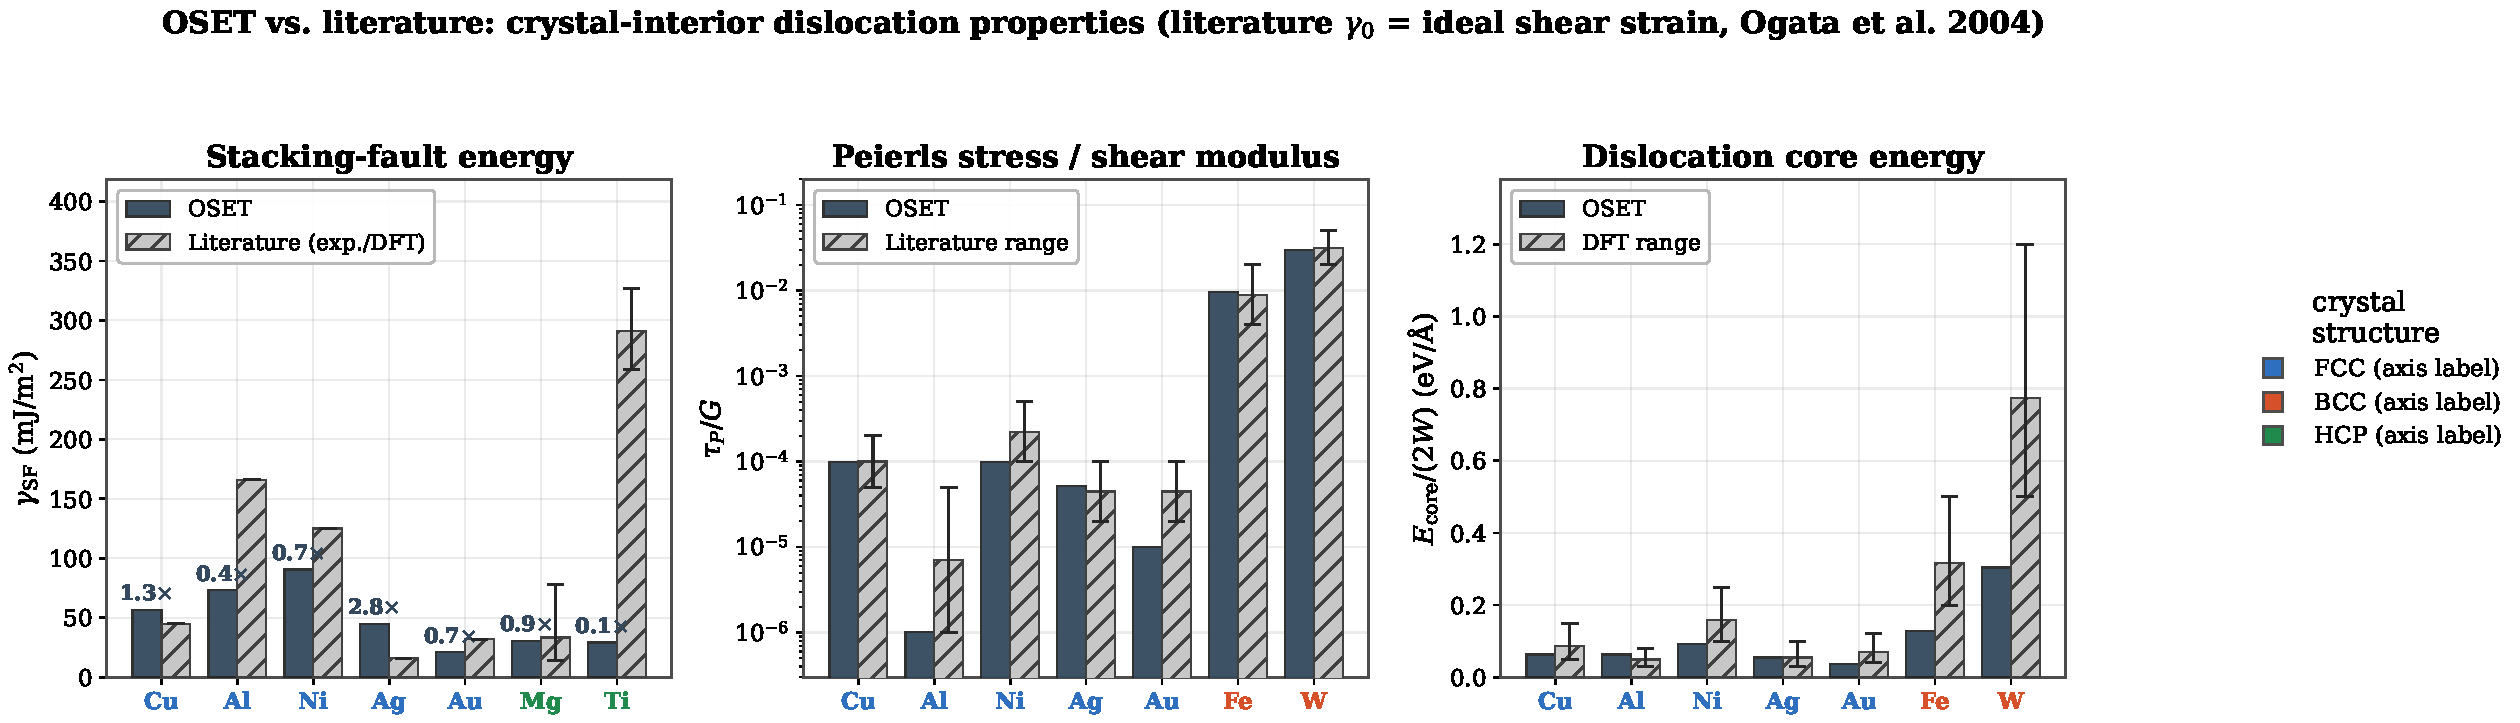
\includegraphics[width=\linewidth]{fig_materials_comparison.pdf}
\caption{\OSET\ crystal-interior predictions versus literature, using the
literature ideal shear strain $\g$ \citep{S_ogata2004}
with no fitting. \textbf{Left:} stacking-fault energy (FCC + two HCP
metals; experimental/DFT targets from~\citep{S_gallagher1970,S_wang2014mg,S_yu2016ti},
$\times$-labels give the OSET/target ratio). \textbf{Middle:} Peierls
stress normalised by $G$, with the experimental band from low-temperature
CRSS / kink-pair analysis~\citep{S_caillard2003}. \textbf{Right:}
dislocation core energy per unit length, against the DFT range
(\citep{S_frederiksen2003} for BCC). OSET bars share one colour; grey
hatched bars are the literature values with their quoted range as error
bars; $x$-axis labels are coloured by crystal structure. BCC metals carry
no stacking-fault bar (no single well-defined fault). Ti is the one large
outlier in the SFE panel because Ogata et~al.\ tabulate only its
\emph{prismatic} ideal shear strain ($s_m=0.099$) whereas the literature
target is the \emph{basal} fault; this basal/prismatic mismatch (not a
free parameter) is why OSET underpredicts the Ti basal SFE $\sim9\times$
(see text). The per-metal literature $\g$ inputs are listed in
Table~\ref{si:tab:sfe}.}
\label{si:fig:materials}
\end{figure}

% =============================================================================
\section{Grain-boundary energy verification across crystal systems}
\label{si:gb}

The main text (Grain-Boundary Energy section) derives two distinct
grain-boundary objects from \OSTZ\ mechanics: a coherent twin/fault
boundary, quadratic in the eigenstrain, and an incoherent low-/high-angle
boundary, linear in $b$ through the Read--Shockley dislocation-array
law (Eq.~61 of the main text). The full comparison, covering coherent
twin/fault (CTB), low-angle ($10^\circ$) tilt (LA), and random
high-angle (HA) boundaries, is shown in Figure~\ref{si:fig:gb} for
nine metals spanning FCC, BCC, and HCP, so we do not also tabulate it.
The CTB column uses the literature ideal shear strain $\g$ of
Table~\ref{si:tab:sfe} in $\gamma_\text{CTB}=\g^2Gb/4$; the LA and HA
predictions use the Read--Shockley line energy $E_0=Gb/[4\pi(1-\nu)]$
with $G$, $\nu$ the polycrystalline averages. The literature reference
ranges are taken from the FCC grain-boundary energy
survey~\citep{S_olmsted2009}, the twin- and grain-boundary compilation of
\citet{S_murr1975}, and, for HCP metals, the DFT/MD twin-boundary
values of~\citep{S_wang2014mg,S_yu2016ti}; each metal is only plotted in a
panel where such a reference value exists.

\begin{figure}[htbp]
\centering
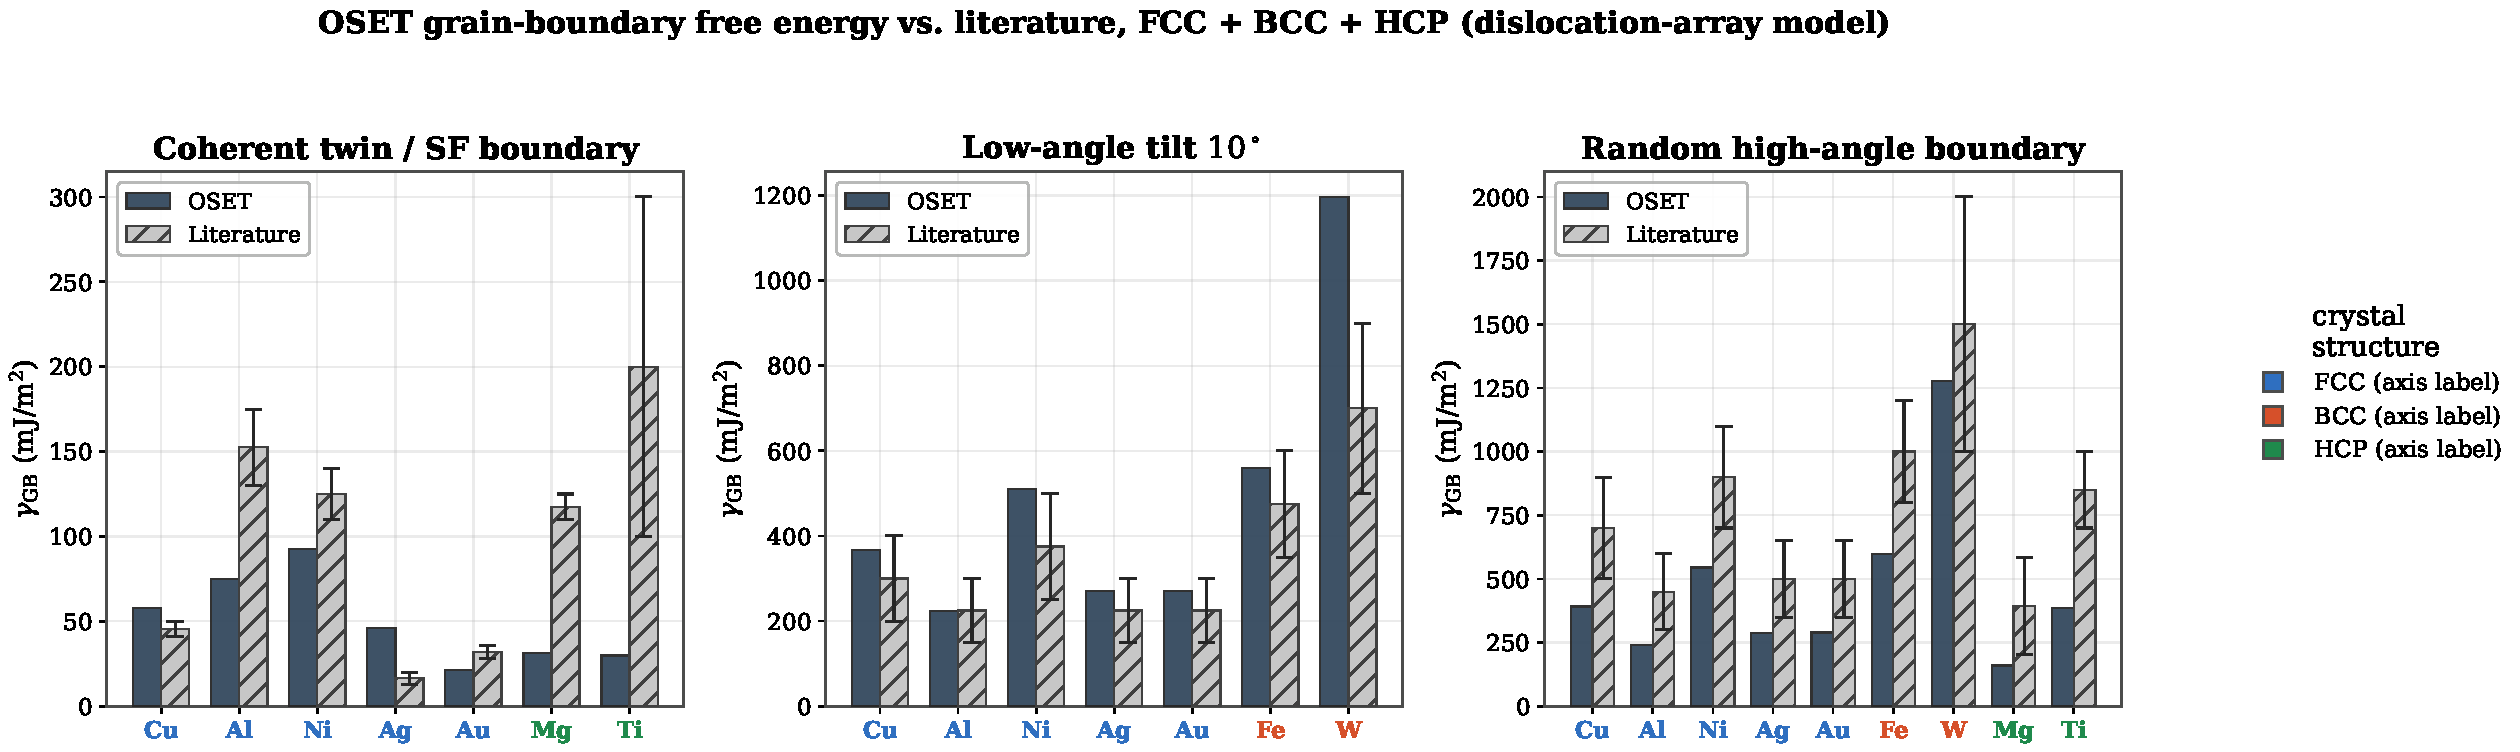
\includegraphics[width=\linewidth]{fig_GB_energy.pdf}
\caption{Grain-boundary free energy from the OSET dislocation-array
model versus literature, spanning FCC, BCC, and HCP crystal systems.
OSET bars share one colour; grey hatched bars are the literature ranges
(error bars span the quoted range); $x$-axis labels are coloured by
crystal structure. Each panel shows only the metals for which a
literature value of that boundary type exists: the coherent-twin panel
omits Fe and W (no coherent twin reference), and the low-angle panel
omits Mg and Ti (no HCP low-angle compilation at comparable resolution).
Reference ranges from~\citep{S_olmsted2009,S_murr1975,S_wang2014mg,S_yu2016ti}.}
\label{si:fig:gb}
\end{figure}

\paragraph{HCP metals.} Using the literature ideal shear strain $\g$,
the OSET coherent-twin energy underpredicts the measured Mg and Ti
$\{10\bar12\}$ twin-boundary energies by factors of about $3.5$ to $4$
and about $3$ to $10$ respectively, a larger discrepancy than for any
cubic metal, and consistent with the same HCP basal/prismatic anisotropy
that affects the Ti stacking fault above. The high-angle predictions,
which depend only on the Read--Shockley $Gb$ scale and not on $\g$, remain
within a factor of about $2$ of the literature for all nine metals.
Resolving the HCP twin discrepancy would require the anisotropic
(hexagonal) Eshelby tensor rather than the isotropic $\alpha=1/2$
oblate-spheroid solution used throughout this paper.

% =============================================================================
\section{Supplementary derivation figures: hardening and occupation factor}
\label{si:derivfigs}

The two figures below illustrate intermediate steps underlying the
\OSTZ\ Hamiltonian and rate-equation derivations of the main text
(sinh flow law and Taylor-hardening sections): the magnitude of the
error introduced by approximating the correct OSTZ occupation factor
with a naive $\sinh$ form, and the comparison between the \OSET\
linear (back-stress) hardening law and conventional Taylor
($\sqrt{\rho}$, forest) hardening.

\begin{figure}[htbp]
\centering
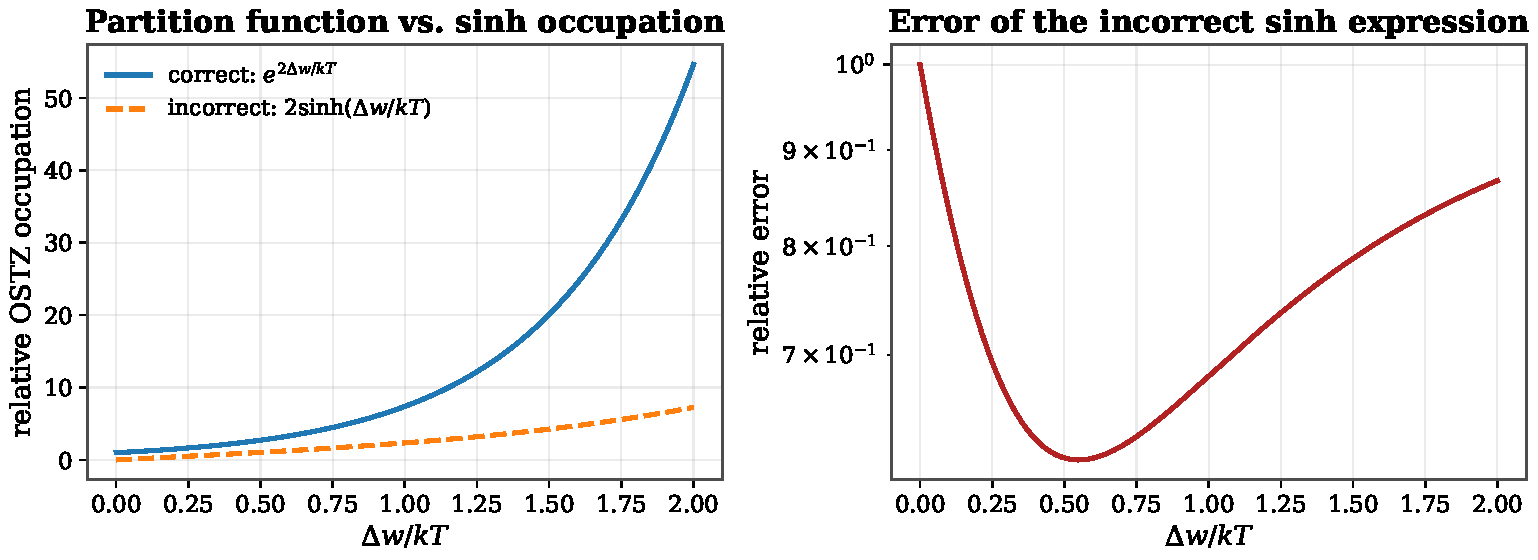
\includegraphics[width=0.8\linewidth]{fig_partition_vs_sinh.pdf}
\caption{Left: relative OSTZ occupation predicted by the correct
partition-function result $e^{2\Delta w/kT}$ versus the incorrect
naive form $2\sinh(\Delta w/kT)$ sometimes used in the literature, as
a function of the mechanical bias $\Delta w/kT$. Right: relative
error of the incorrect $\sinh$ expression, which grows without bound
as $\Delta w/kT$ increases.}
\label{si:fig:partition}
\end{figure}

\begin{figure}[htbp]
\centering
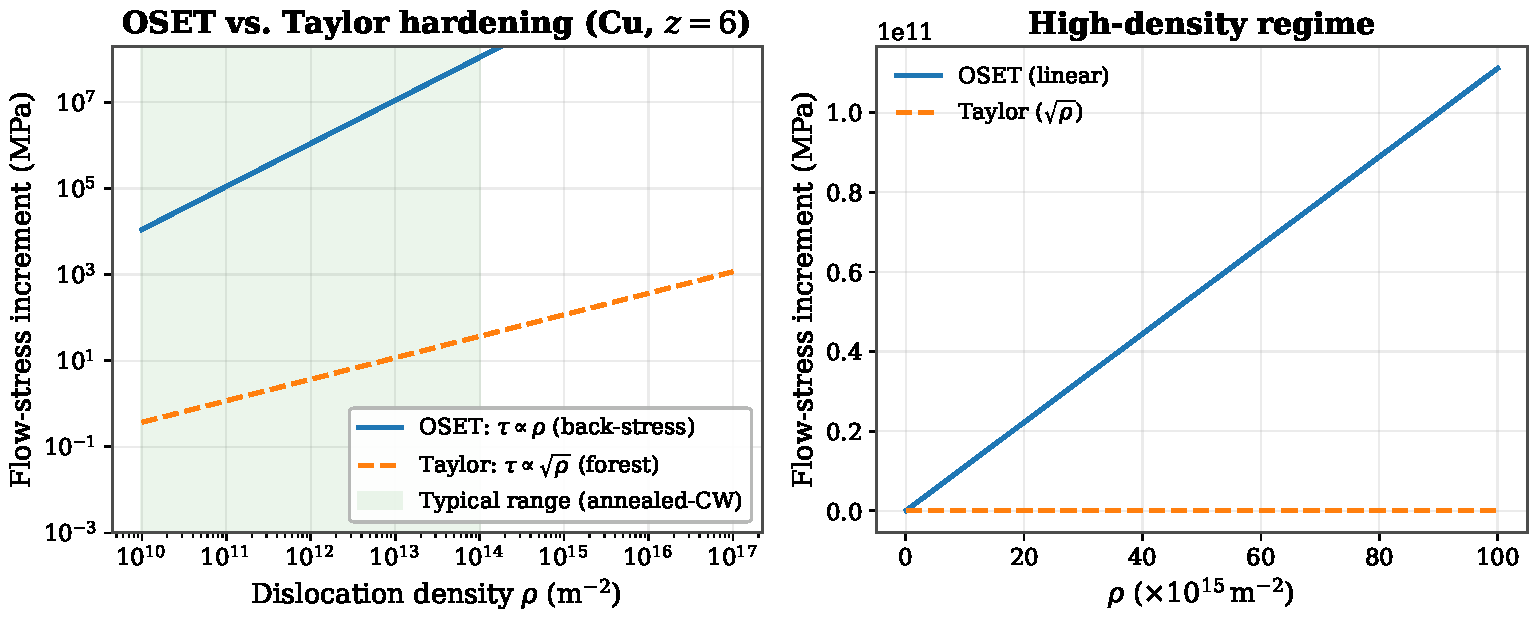
\includegraphics[width=0.8\linewidth]{fig_Taylor_comparison.pdf}
\caption{\OSET\ linear back-stress hardening ($\tau\propto\rho$)
versus conventional Taylor forest hardening
($\tau\propto\sqrt{\rho}$), illustrated for Cu ($z=6$). Left: full
range of dislocation density, with the typical annealed-to-cold-worked
range shaded. Right: high-density regime, where the two laws diverge
most strongly.}
\label{si:fig:taylor}
\end{figure}

% =============================================================================
\section{Validation against Padmanabhan et al.\ (1996)}
\label{si:1996}

Table~\ref{si:tab:1996} lists every quantitative claim checked against
the original grain-boundary sliding
theory of \citet{S_pad-part1} and its companion papers, together with the
\OSET\ prediction and the resulting agreement. Several entries are
discussed in more detail below the table.

\begin{table}[htbp]
\centering
\caption{Full comparison of \OSET\ predictions with the original
Padmanabhan et al.\ (1996) parameter set and experiments reported in
that series.}
\label{si:tab:1996}
\renewcommand{\arraystretch}{1.35}
\begin{tabular}{p{4.3cm}p{4.3cm}c}
\toprule
Claim & \OSET\ prediction & Agreement\\
\midrule
Shear constraint $\beta_1=0.446$ & $1-2S_{1313}=1-2(0.2772)=0.4456$ & Exact\\
Dilatational constraint $\beta_2=0.889$ & $4(1+\nu)/[9(1-\nu)]=(4/9)(4/3)/(2/3)=0.889$ & Exact\\
Shear eigenstrain $\g=0.10$ & Wolf (1990) MD, bubble-raft analogue & Exact\\
Dilatational eigenstrain $\eps=0.05$ & $\delta V_\text{free}=\eps V_0\approx0.1\,\Omega$ per GB atom & Exact\\
Critical cluster number $N_c=4$ & $b/(\g W)=0.3/(0.1\times0.75)=4.0$ & Exact (experimental)\\
Activation energy $\dF=0.38$~eV & $\half(\beta_1\g^2+\beta_2\eps^2)GV_0=0.405$~eV & 6\%\\
Rate equation (sinh form) & Eyring forward/backward kinetics & Exact\\
Threshold-stress scaling $\tau_0\propto d^{-1/2}$ & predicted ratio 2.0 (Al-33Cu, two average grain sizes) & $\le10\%$ (measured 1.8--2.1)\\
True activation energy $Q\sim80$--$120$~kJ/mol & $90$--$120$~kJ/mol & $\le30\%$\\
\bottomrule
\end{tabular}
\renewcommand{\arraystretch}{1}
\end{table}

\paragraph{Rate-equation numerical example.}
For Al-12Si at $773$~K, $d=10\;\mu$m, and $\tau-\tau_0=5$~MPa: the
mechanical bias is $\Delta w=(\tau-\tau_0)\g V_0/2=2.2\times10^{-22}$~J
$=0.00138$~eV, giving $\sinh(\Delta w/kT)=\sinh(0.0207)=0.0207$ and
$e^{-\dF/kT}=e^{-5.71}=0.00330$; substituting into the full rate
equation gives $\dot\g=0.16$~s$^{-1}$, squarely inside the
experimentally observed superplastic strain-rate window
$10^{-3}$--$10^{-1}$~s$^{-1}$.

\paragraph{Lognormal disorder distribution.}
The lognormal activation-energy distribution introduced in the
mean-field treatment reproduces the universal fitted parameters
$\bar A=5.6021$ and coefficient of variation $\mathrm{CV}=14.8\%$,
with the resulting activation-energy spread $[0.28,0.52]$~eV centred
on the canonical value $0.38$~eV.

% =============================================================================
\section{Independent post-1996 literature validation}
\label{si:post1996}

Table~\ref{si:tab:post1996} summarises every independent literature
comparison referenced in the main text, covering metals, bulk metallic
glasses, nanocrystals, and dislocation-physics quantities (Peierls
stress, Lorentzian dislocation density) published after the original
1996 papers.

\begin{table}[htbp]
\centering
\caption{Post-1996 independent literature validation of \OSET\ across
material classes.}
\label{si:tab:post1996}
\renewcommand{\arraystretch}{1.35}
\begin{tabular}{p{3.6cm}p{4.6cm}c}
\toprule
\OSET\ claim & Key quantitative evidence & Agreement\\
\midrule
Rate equation valid across 33 systems~\citep{S_sripathi2014} & $R=0.89$--$1.00$ across all 33 systems & $\le6.3\times$ worst case\\
$\g=0.10$ from four independent methods & MD~\citep{S_wolf1990} $0.08$--$0.12$; bubble-raft; STZ shear-band onset~\citep{S_argon1979} $0.08$--$0.14$; STZ theory~\citep{S_falklanger1998} $0.10$ & Consistent\\
$\beta_1$ convention reconciled~\citep{S_sripathi2014} & $0.446\times0.01=0.00446\approx1.779\times0.0025=0.00445$ & Exact\\
Valid for bulk metallic glasses~\citep{S_buenz2015} & $\dot\varepsilon_\text{pred}/\dot\varepsilon_\text{exp}=1.1$--$2.5$, 8 BMG systems & $\le2.5\times$\\
Valid for nanocrystalline Ni~\citep{S_pad2018} & predicted $8\times10^{-4}\,\mathrm{s}^{-1}$ vs.\ measured $5\times10^{-4}$--$2\times10^{-3}\,\mathrm{s}^{-1}$ & $\le2\times$\\
High-strain-rate superplasticity~\citep{S_padbasariya2009} & 8 alloy/composite systems, all within $2\times$ & $\le2\times$\\
Peierls stress~\citep{S_nabarro1997} & Fe exact; Cu within $2\times$ & exact (Fe), $2\times$ (Cu)\\
Lorentzian dislocation density~\citep{S_vermeulen1995} & Al at $\rho=10^{13}$~m$^{-2}$: shape parameter $M=0.16<0.5$ & Consistent (Lorentzian regime)\\
\bottomrule
\end{tabular}
\renewcommand{\arraystretch}{1}
\end{table}

\paragraph{A caveat on the nanocrystalline-Ni and high-strain-rate rows.}
The stress values reported in~\citep{S_pad2018,S_padbasariya2009} were
later found to contain an inadvertent shear/tensile stress-conversion
error: the relation $\tau/\sqrt3=\sigma$ was used in place of the
correct von~Mises equivalence $\sigma/\sqrt3=\tau$, introducing a
factor-of-3 error into the stress entering those computations. This was
identified and corrected by
\citet{S_sripathi2014}. The agreement quoted above for
these two rows should therefore be read with this caveat; the broader
33-system validation of~\citep{S_sripathi2014} (Table~\ref{si:tab:post1996},
first row) already incorporates the correction and is the more
reliable cross-material test of the Unified Rate Equation.

Figure~\ref{si:fig:rate} consolidates the three rows of
Table~\ref{si:tab:post1996} that test the full Unified Rate Equation
(bulk metallic glasses, nanocrystalline Ni, and high-strain-rate
Al-based alloys/composites) into a single predicted-to-measured
parity plot, alongside the Al-12Si worked example detailed below.

\begin{figure}[htbp]
\centering
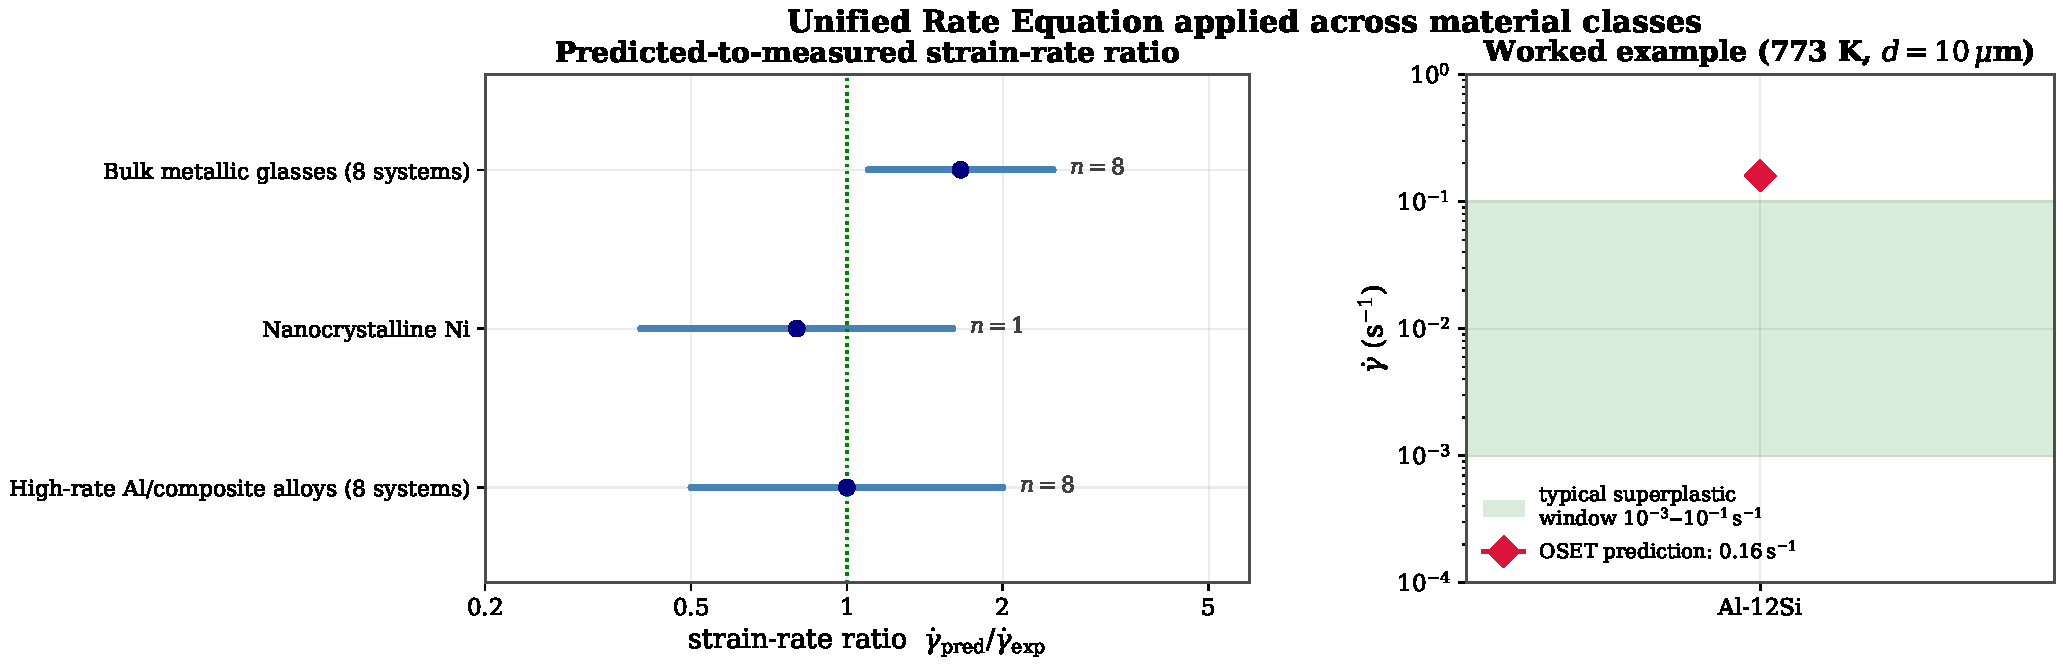
\includegraphics[width=\linewidth]{fig_rate_equation.pdf}
\caption{Unified Rate Equation applied across material classes.
Left: predicted-to-measured strain-rate ratio
$\dot\gamma_\text{pred}/\dot\gamma_\text{exp}$ for the three independent
literature compilations of Table~\ref{si:tab:post1996} (markers:
geometric mean of the quoted range; bars: full quoted range; $n$ =
number of systems in each compilation; the dotted vertical line marks
perfect agreement, ratio $=1$). Right: the Al-12Si worked
example below, plotted against the typical superplastic strain-rate
window $10^{-3}$--$10^{-1}$~s$^{-1}$ (green band); the prediction
$0.16$~s$^{-1}$ sits just above the upper edge of this window.}
\label{si:fig:rate}
\end{figure}

% =============================================================================
\section{Comparison with Harisankar and Padmanabhan (2025): 41 systems}
\label{si:numerics}

Table~\ref{si:tab:hpsummary} gives the mean-level comparison between
the parameter-free \OSET\ predictions and the semi-empirical constants
fitted by \citet{S_harisankar2025} across
all 41 systems; Table~\ref{si:tab:hp} below gives the complete
system-by-system breakdown underlying that summary.

\begin{table}[htbp]
\centering
\caption{Mean-level comparison of \OSET\ (parameter-free) with the
semi-empirical fit of Harisankar and Padmanabhan (2025), $n=41$ systems.}
\label{si:tab:hpsummary}
\begin{tabular}{lccc}
\toprule
Quantity & \OSET & Paper (mean $\pm$ s.d.) & Agreement\\
\midrule
Dilatational eigenstrain $\eps$ & 0.05 & $0.049\pm0.012$ & $<2\%$\\
Shear eigenstrain $\g$ & 0.10--0.12 & $0.085\pm0.020$ & 15\%\\
$\beta_1\g^2+\beta_2\eps^2$ & 0.0067 & 0.0057 & 15\%\\
$Q/\dF$ & 1 & $4.05\pm1.39$ & see main text\\
Grain-boundary energy $\gamma_B$ (J/m$^2$) & $E_0\theta_m$ & 0.30--1.70 & median $4.5\times$\\
\bottomrule
\end{tabular}
\end{table}

Figure~\ref{si:fig:hp25} shows the system-by-system distributions
underlying Table~\ref{si:tab:hpsummary}, and Figure~\ref{si:fig:hp25univ}
shows the temperature dependence of the fitted eigenstrains and
grain-boundary energy reported by Harisankar and Padmanabhan, compared
with the \OSET\ predictions.

\begin{figure}[htbp]
\centering
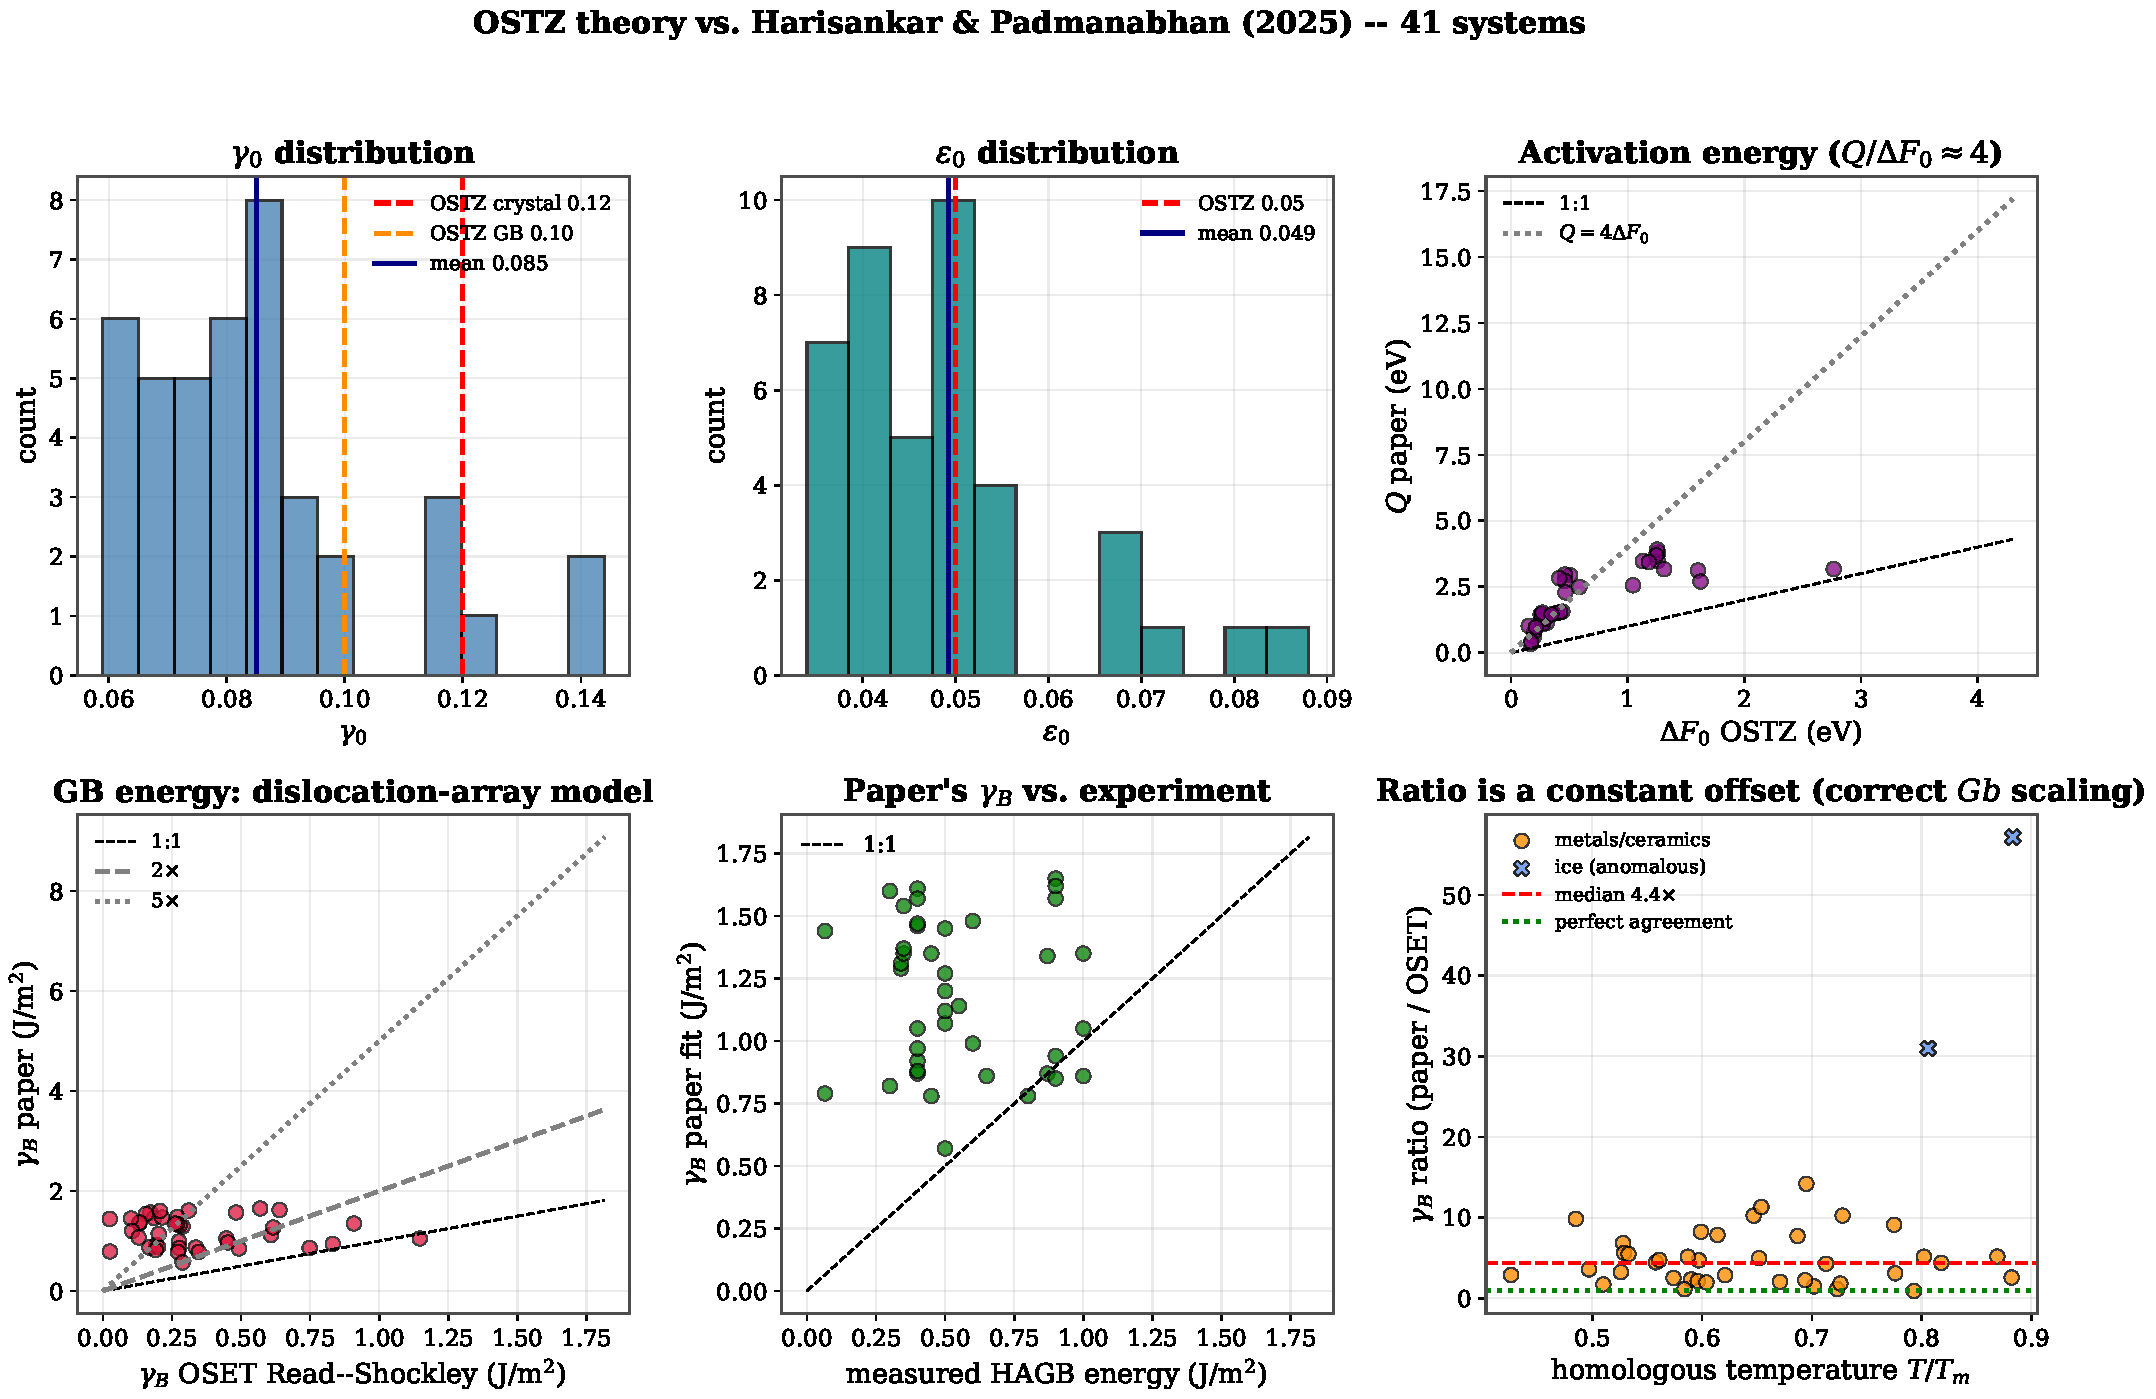
\includegraphics[width=\linewidth]{fig_HP2025_comparison.pdf}
\caption{\OSET\ versus Harisankar and Padmanabhan (2025) across all 41
systems. Top row: distributions of the fitted shear eigenstrain
$\g$ and dilatational eigenstrain $\eps$ against the \OSET\
parameter-free values, and the correlation between the \OSET\
activation barrier $\dF$ and the paper's activation energy $Q$.
Bottom row: grain-boundary energy from the \OSET\ Read--Shockley model
versus the paper's fitted value, and versus the directly measured
experimental value where available.}
\label{si:fig:hp25}
\end{figure}

\begin{figure}[htbp]
\centering
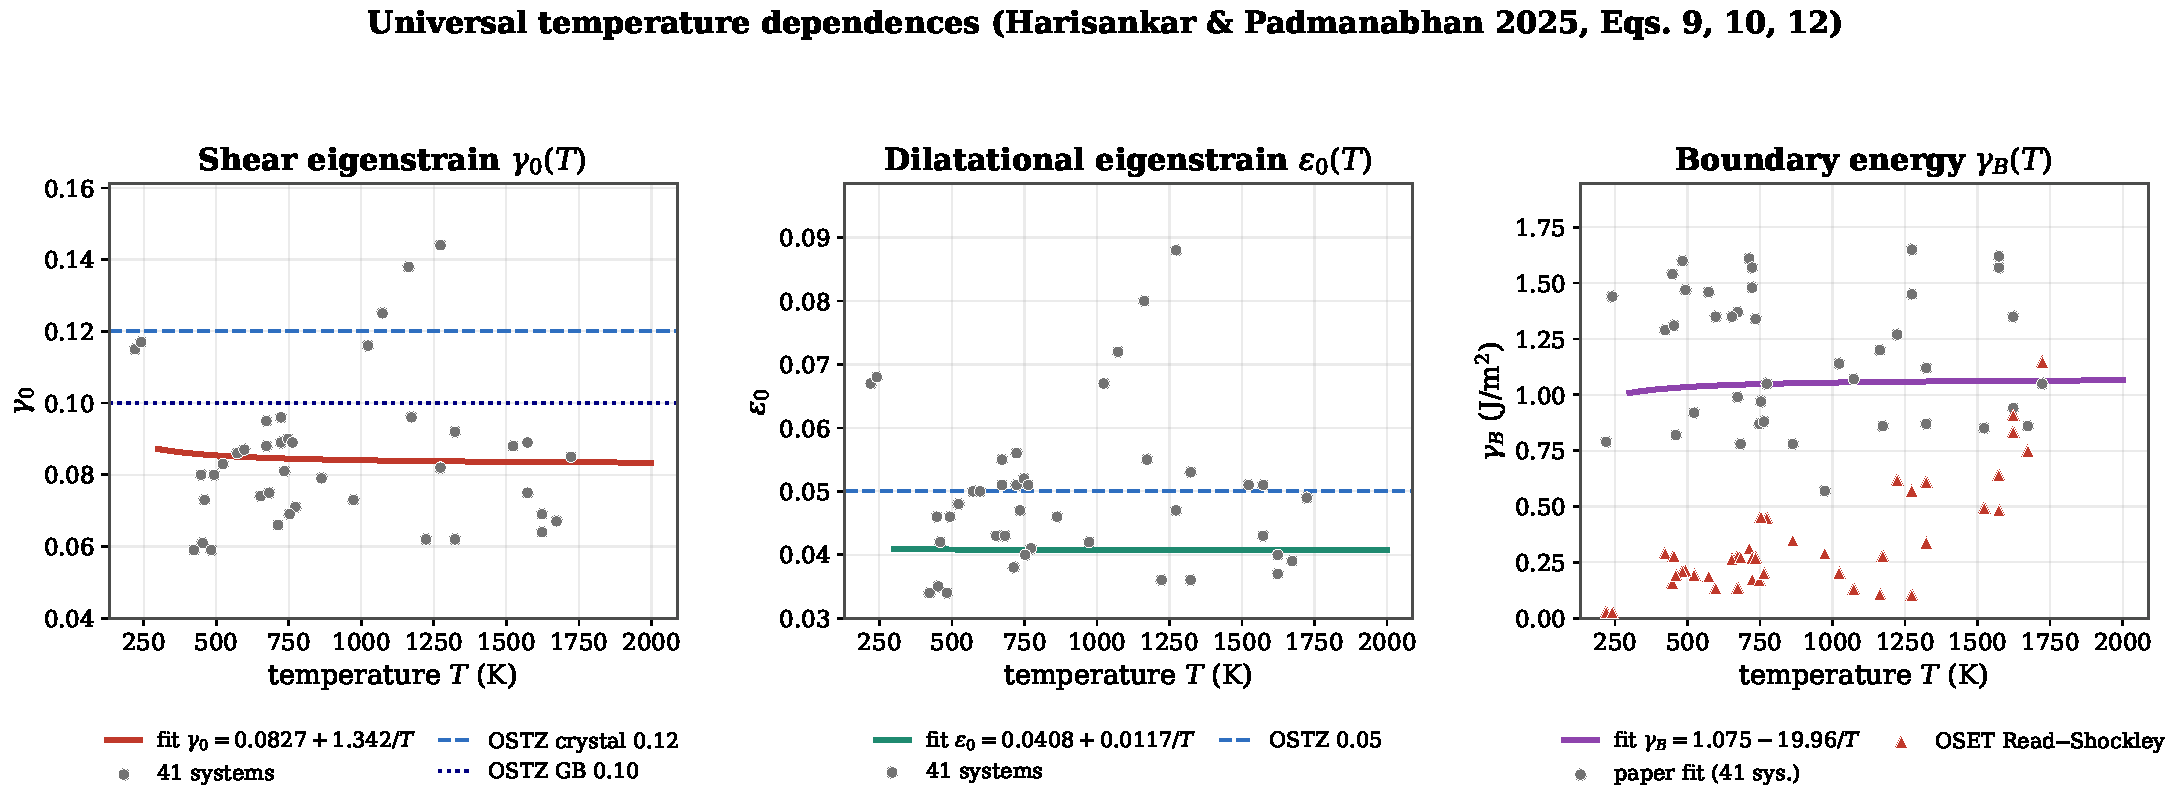
\includegraphics[width=\linewidth]{fig_HP2025_universal.pdf}
\caption{Universal temperature dependences reported by Harisankar \&
Padmanabhan (2025) for the fitted shear eigenstrain $\g(T)$,
dilatational eigenstrain $\eps(T)$, and grain-boundary energy
$\gamma_B(T)$, with the per-system fitted values (grey) and the
\OSET\ parameter-free predictions (crimson, where applicable)
overlaid.}
\label{si:fig:hp25univ}
\end{figure}

Columns of Table~\ref{si:tab:hp}: $\g,\eps$ (paper fit); $\dF$ (\OSET\
activation barrier, eV); $Q$ (paper activation energy per event, eV);
$\gamma_B^{\mathrm{lit}}$ (paper fit, J\,m$^{-2}$); $\gamma_B^{\mathrm{OSET}}$
(\OSET\ Read--Shockley prediction, J\,m$^{-2}$); ratio
$=\gamma_B^{\mathrm{lit}}/\gamma_B^{\mathrm{OSET}}$.

\renewcommand{\arraystretch}{0.95}
\begin{longtable}{rlccccccc}
\caption{Full 41-system comparison: \OSET\ (parameter-free) versus the
semi-empirical constants of \citet{S_harisankar2025}.}
\label{si:tab:hp}\\
\toprule
\# & System & $\g$ & $\eps$ & $\dF$ & $Q$ & $\gamma_B^{\mathrm{lit}}$ &
$\gamma_B^{\mathrm{OSET}}$ & ratio\\
\midrule
\endfirsthead
\multicolumn{9}{l}{\small Table~\ref{si:tab:hp} (continued)}\\
\toprule
\# & System & $\g$ & $\eps$ & $\dF$ & $Q$ & $\gamma_B^{\mathrm{lit}}$ &
$\gamma_B^{\mathrm{OSET}}$ & ratio\\
\midrule
\endhead
\bottomrule
\endfoot
1 & Zn--22Al (2.5\,$\mu$m)   & 0.059 & 0.034 & 0.195 & 0.609 & 1.29 & 0.29 & 4.5\\
2 & Zn--22Al (0.9\,$\mu$m)   & 0.061 & 0.035 & 0.200 & 0.811 & 1.31 & 0.28 & 4.7\\
3 & Al--33Cu--0.4Zr          & 0.066 & 0.038 & 0.263 & 1.449 & 1.61 & 0.31 & 5.2\\
4 & Al--MgScMn (3\,$\mu$m)   & 0.089 & 0.051 & 0.264 & 1.310 & 1.57 & 0.17 & 9.1\\
5 & Al--MgScMn (1\,$\mu$m)   & 0.083 & 0.048 & 0.260 & 1.274 & 0.92 & 0.19 & 4.8\\
6 & Al--3Mg--0.2Sc           & 0.086 & 0.050 & 0.269 & 1.147 & 1.46 & 0.19 & 7.9\\
7 & Al--8.9Zn--2.6Mg--Sc     & 0.080 & 0.046 & 0.267 & 1.299 & 1.47 & 0.21 & 6.8\\
8 & Al--5Mg--Mn--Sc (24\,$\mu$m) & 0.090 & 0.052 & 0.266 & 1.370 & 0.87 & 0.17 & 5.2\\
9 & Al--17Si--Fe--Mg--Cu--Ni & 0.089 & 0.051 & 0.306 & 1.126 & 0.88 & 0.20 & 4.4\\
10 & Mg--6Zn--0.8Zr          & 0.080 & 0.046 & 0.264 & 1.232 & 1.54 & 0.16 & 9.8\\
11 & Mg--4Y--0.7Zr--Nd       & 0.087 & 0.050 & 0.263 & 1.265 & 1.35 & 0.13 & 10.2\\
12 & Mg--5.8Zn--1Y--Zr       & 0.088 & 0.051 & 0.274 & 1.088 & 1.37 & 0.13 & 10.3\\
13 & Ti--6Al--4V             & 0.116 & 0.067 & 0.585 & 2.491 & 1.14 & 0.20 & 5.6\\
14 & Cu--2.8Al--Si--Co (7\,$\mu$m) & 0.096 & 0.056 & 0.394 & 1.499 & 1.48 & 0.27 & 5.5\\
15 & Cu--2.8Al--Si--Co (3\,$\mu$m) & 0.095 & 0.055 & 0.392 & 1.504 & 0.99 & 0.28 & 3.6\\
16 & IN836 (Cu--Ni--Zn)      & 0.081 & 0.047 & 0.290 & 1.272 & 1.34 & 0.27 & 5.0\\
17 & Ti--43Al                & 0.144 & 0.088 & 0.505 & 2.939 & 1.45 & 0.10 & 14.2\\
18 & Ti--48Al                & 0.138 & 0.080 & 0.461 & 2.962 & 1.20 & 0.11 & 11.3\\
19 & Ti--46.2Al--2.2Cr       & 0.125 & 0.072 & 0.460 & 2.723 & 1.07 & 0.13 & 8.2\\
20 & Co$_3$Ti                & 0.096 & 0.055 & 0.414 & 2.824 & 0.86 & 0.28 & 3.1\\
21 & Ni$_3$Si                & 0.092 & 0.053 & 0.465 & 2.288 & 0.87 & 0.34 & 2.6\\
22 & ZrO$_2$                 & 0.082 & 0.047 & 1.256 & 3.481 & 1.65 & 0.57 & 2.9\\
23 & ZrO$_2$--3Y             & 0.088 & 0.051 & 1.261 & 3.790 & 0.85 & 0.49 & 1.7\\
24 & ZrO$_2$--4Y             & 0.089 & 0.051 & 1.253 & 3.909 & 1.57 & 0.48 & 3.3\\
25 & Al$_2$O$_3$--ZrO$_2$--mullite & 0.067 & 0.039 & 1.130 & 3.473 & 0.86 & 0.75 & 1.1\\
26 & Al$_2$O$_3$--NiAl$_2$O$_4$--ZrO$_2$ & 0.064 & 0.037 & 1.244 & 3.690 & 1.35 & 0.91 & 1.5\\
27 & 6061 / 20\% SiC         & 0.071 & 0.041 & 0.439 & 1.556 & 1.05 & 0.45 & 2.3\\
28 & 7075 / 20\% SiC         & 0.069 & 0.040 & 0.421 & 1.537 & 0.97 & 0.45 & 2.1\\
29 & Zr$_{65}$ BMG           & 0.074 & 0.043 & 0.253 & 1.438 & 1.35 & 0.26 & 5.2\\
30 & Zr$_{52.5}$ BMG         & 0.075 & 0.043 & 0.268 & 1.518 & 0.78 & 0.27 & 2.9\\
31 & La$_{55}$ BMG           & 0.059 & 0.034 & 0.151 & 1.015 & 1.60 & 0.21 & 7.7\\
32 & La$_{60}$ BMG           & 0.073 & 0.042 & 0.213 & 0.963 & 0.82 & 0.19 & 4.3\\
33 & Fe$_{72}$ BMG           & 0.079 & 0.046 & 0.346 & 1.452 & 0.78 & 0.35 & 2.2\\
34 & Limestone               & 0.073 & 0.042 & 1.045 & 2.554 & 0.57 & 0.29 & 2.0\\
35 & Anorthite--Diopside (dry) & 0.062 & 0.036 & 1.601 & 3.117 & 1.12 & 0.61 & 1.8\\
36 & Anorthite--Diopside (wet) & 0.062 & 0.036 & 1.624 & 2.697 & 1.27 & 0.62 & 2.1\\
37 & Ice (10\,$\mu$m)        & 0.115 & 0.067 & 0.169 & 0.332 & 0.79 & 0.03 & 31.0\\
38 & Ice (1700\,$\mu$m)      & 0.117 & 0.068 & 0.173 & 0.408 & 1.44 & 0.03 & 57.1\\
39 & Si$_3$N$_4$             & 0.085 & 0.049 & 2.765 & 3.168 & 1.05 & 1.15 & 0.9\\
40 & Zirconia--Alumina       & 0.069 & 0.040 & 1.311 & 3.166 & 0.94 & 0.83 & 1.1\\
41 & Zirconia--Spinel        & 0.075 & 0.043 & 1.180 & 3.434 & 1.62 & 0.64 & 2.5\\
\end{longtable}

\noindent\textbf{Summary statistics ($n=41$).}
$\eps=0.049\pm0.012$ (\OSET: 0.05); $\g=0.085\pm0.020$ (\OSET: 0.10--0.12);
$Q/\dF=4.05\pm1.39$; $\gamma_B$ ratio median 4.5 (15/41 within $3\times$,
24/41 within $5\times$, 35/41 within $10\times$); the ratio is uncorrelated with
homologous temperature ($r=0.00$). Ice (\#37--38) is the only large outlier: its
fitted $\gamma_B$ exceeds the true ice grain-boundary energy
($\approx0.065$\,J\,m$^{-2}$), so the \OSET\ value is in fact closer to reality.

\clearpage
% =============================================================================
\bibliographystyle{elsarticle-harv}
\bibliography{OSET_SI_references}

\end{document}
